\documentclass[10pt,landscape]{article}
\usepackage{multicol,multirow}
\usepackage{calc}
\usepackage{ifthen}
\usepackage[landscape]{geometry}
\usepackage[colorlinks=true,citecolor=blue,linkcolor=blue]{hyperref}
\usepackage[fleqn]{amsmath}
\usepackage{amssymb,amsthm,amsfonts}
\usepackage{graphicx}
\usepackage{wrapfig}
\usepackage{cancel}

\ifthenelse{\lengthtest { \paperwidth = 11in}}
{ \geometry{top=.3in,left=.3in,right=.3in,bottom=.3in} }
{\ifthenelse{ \lengthtest{ \paperwidth = 297mm}}
{\geometry{top=1cm,left=1cm,right=1cm,bottom=1cm} }
{\geometry{top=1cm,left=1cm,right=1cm,bottom=1cm} }
}
\pagestyle{empty}
\makeatletter
\renewcommand{\section}{\@startsection{section}{1}{0mm}%
{-1ex plus -.5ex minus -.2ex}%
{0.5ex plus .2ex}%x
{\normalfont\large\bfseries}}
\renewcommand{\subsection}{\@startsection{subsection}{2}{0mm}%
{-1explus -.5ex minus -.2ex}%
{0.5ex plus .2ex}%
{\normalfont\normalsize\bfseries}}
\renewcommand{\subsubsection}{\@startsection{subsubsection}{3}{0mm}%
{-1ex plus -.5ex minus -.2ex}%
{1ex plus .2ex}%
{\normalfont\small\bfseries}}
\renewcommand{\arraystretch}{1.3}
\makeatother
\setcounter{secnumdepth}{0}
\setlength{\parindent}{0pt}
\setlength{\parskip}{0pt plus 0.5ex}
\setlength{\mathindent}{0pt}
\setlength{\columnseprule}{0.2pt}
% -----------------------------------------------------------------------

\title{Numerical Analysis and Computer Algebra}

\begin{document}
    \raggedright
    \footnotesize

    \begin{center}
        \textbf{Partial Differential Equations} \\
    \end{center}
    \begin{multicols}{3}
        \setlength{\premulticols}{1pt}
        \setlength{\postmulticols}{1pt}
        \setlength{\multicolsep}{1pt}
        \setlength{\columnsep}{2pt}

        \section{Newton Polynomial Interpolation}

For some interpolation problem (collocation), a polynomial 
$p(x) = c_0 + c_1x + c_2x^2 + \ldots + c_mx^m$
of degree $m$ is required such that the degree $m$ is minimal while meeting collocation conditions.

The data (measurements) are given by indexed pairs $(x_k,y_k)$ with $k=0,1,2,\ldots,n$.

\subsection{Aitken-Neville Recursion Formula}

Group together polynomials of a subset of the measurement into a global polynomial, e.g. for a dataset with three measurements:

\begin{align*}
	p_{0,1,2}(x)=\frac{(x-x_0)p_{1,2}(x) - (x-x_2)p_{0,1}(x)}{(x_2-x_0)}
\end{align*}

\subsection{Newton Basis Polynomials}

The basis polynomials with degree $k=0,1,2,\ldots,n$:

\begin{snugshade*}
	\begin{align*}
		\pi_0(x) & = 1 \\
		\pi_1(x) & = (x-x_0) \\ 
		\pi_2(x) & = (x-x_0)(x-x_1) \\
		\vdots \\
		\pi_n(x) & = (x-x_0)(x-x_1)\ldots(x-x_{n-1})
	\end{align*}
\end{snugshade*}

can be used to form a collocation polynomial using a linear combination 
$p(x)=a_0\pi_0(x) + a_1\pi_1(x) + \ldots + a_m\pi_m(x)$. 
This forms the system of linear equations
\begin{align*}
	y_0 & = a_0 \\
	y_1 & = a_0 + a_1(x_1-x_0) \\
	y_2 & = a_0 + a_1(x_1-x_0) + a_2(x_2-x_0)(x_2-x_1) \\
	\vdots \\
	y_n & = a_0+a_1\pi_1(x_n)+a_2\pi_2(x_n)+\ldots+a_n\pi_n(x_n)
\end{align*}

\emph{Stability}: Since the coefficient $a_k$ is determined by the first $k$ arguments,
we can extend the dataset with new data without altering existing coefficients.

\subsubsection{Divided Differences}

Due to stability, we can write the coefficients as $a_k(x_0,\ldots,x_k)$, only depending on the arguments lower than $k$.
Applying the Aitken-Neville formula, we receive for $k=0,1,\ldots,n$:

\begin{align*}
	y(x_0, x_2, \ldots, x_k)=\frac{y(x_1,x_2,\ldots,x_k) - y(x_0, x_1, \ldots, x_{k-1})}{(x_k - x_0)}
\end{align*}

\makebox[\columnwidth]{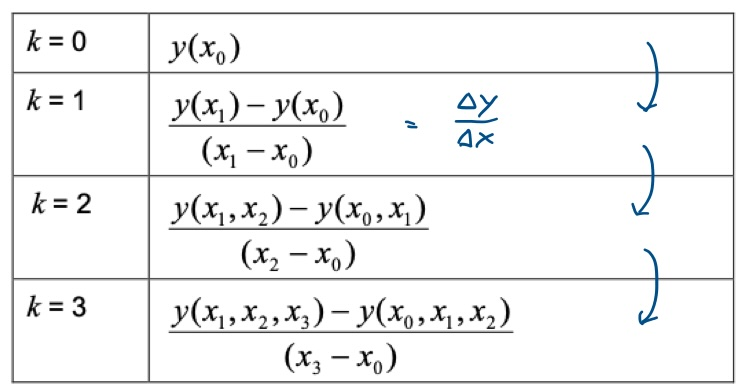
\includegraphics[width=0.6\columnwidth]{images/aitken-neville}}

\makebox[\columnwidth]{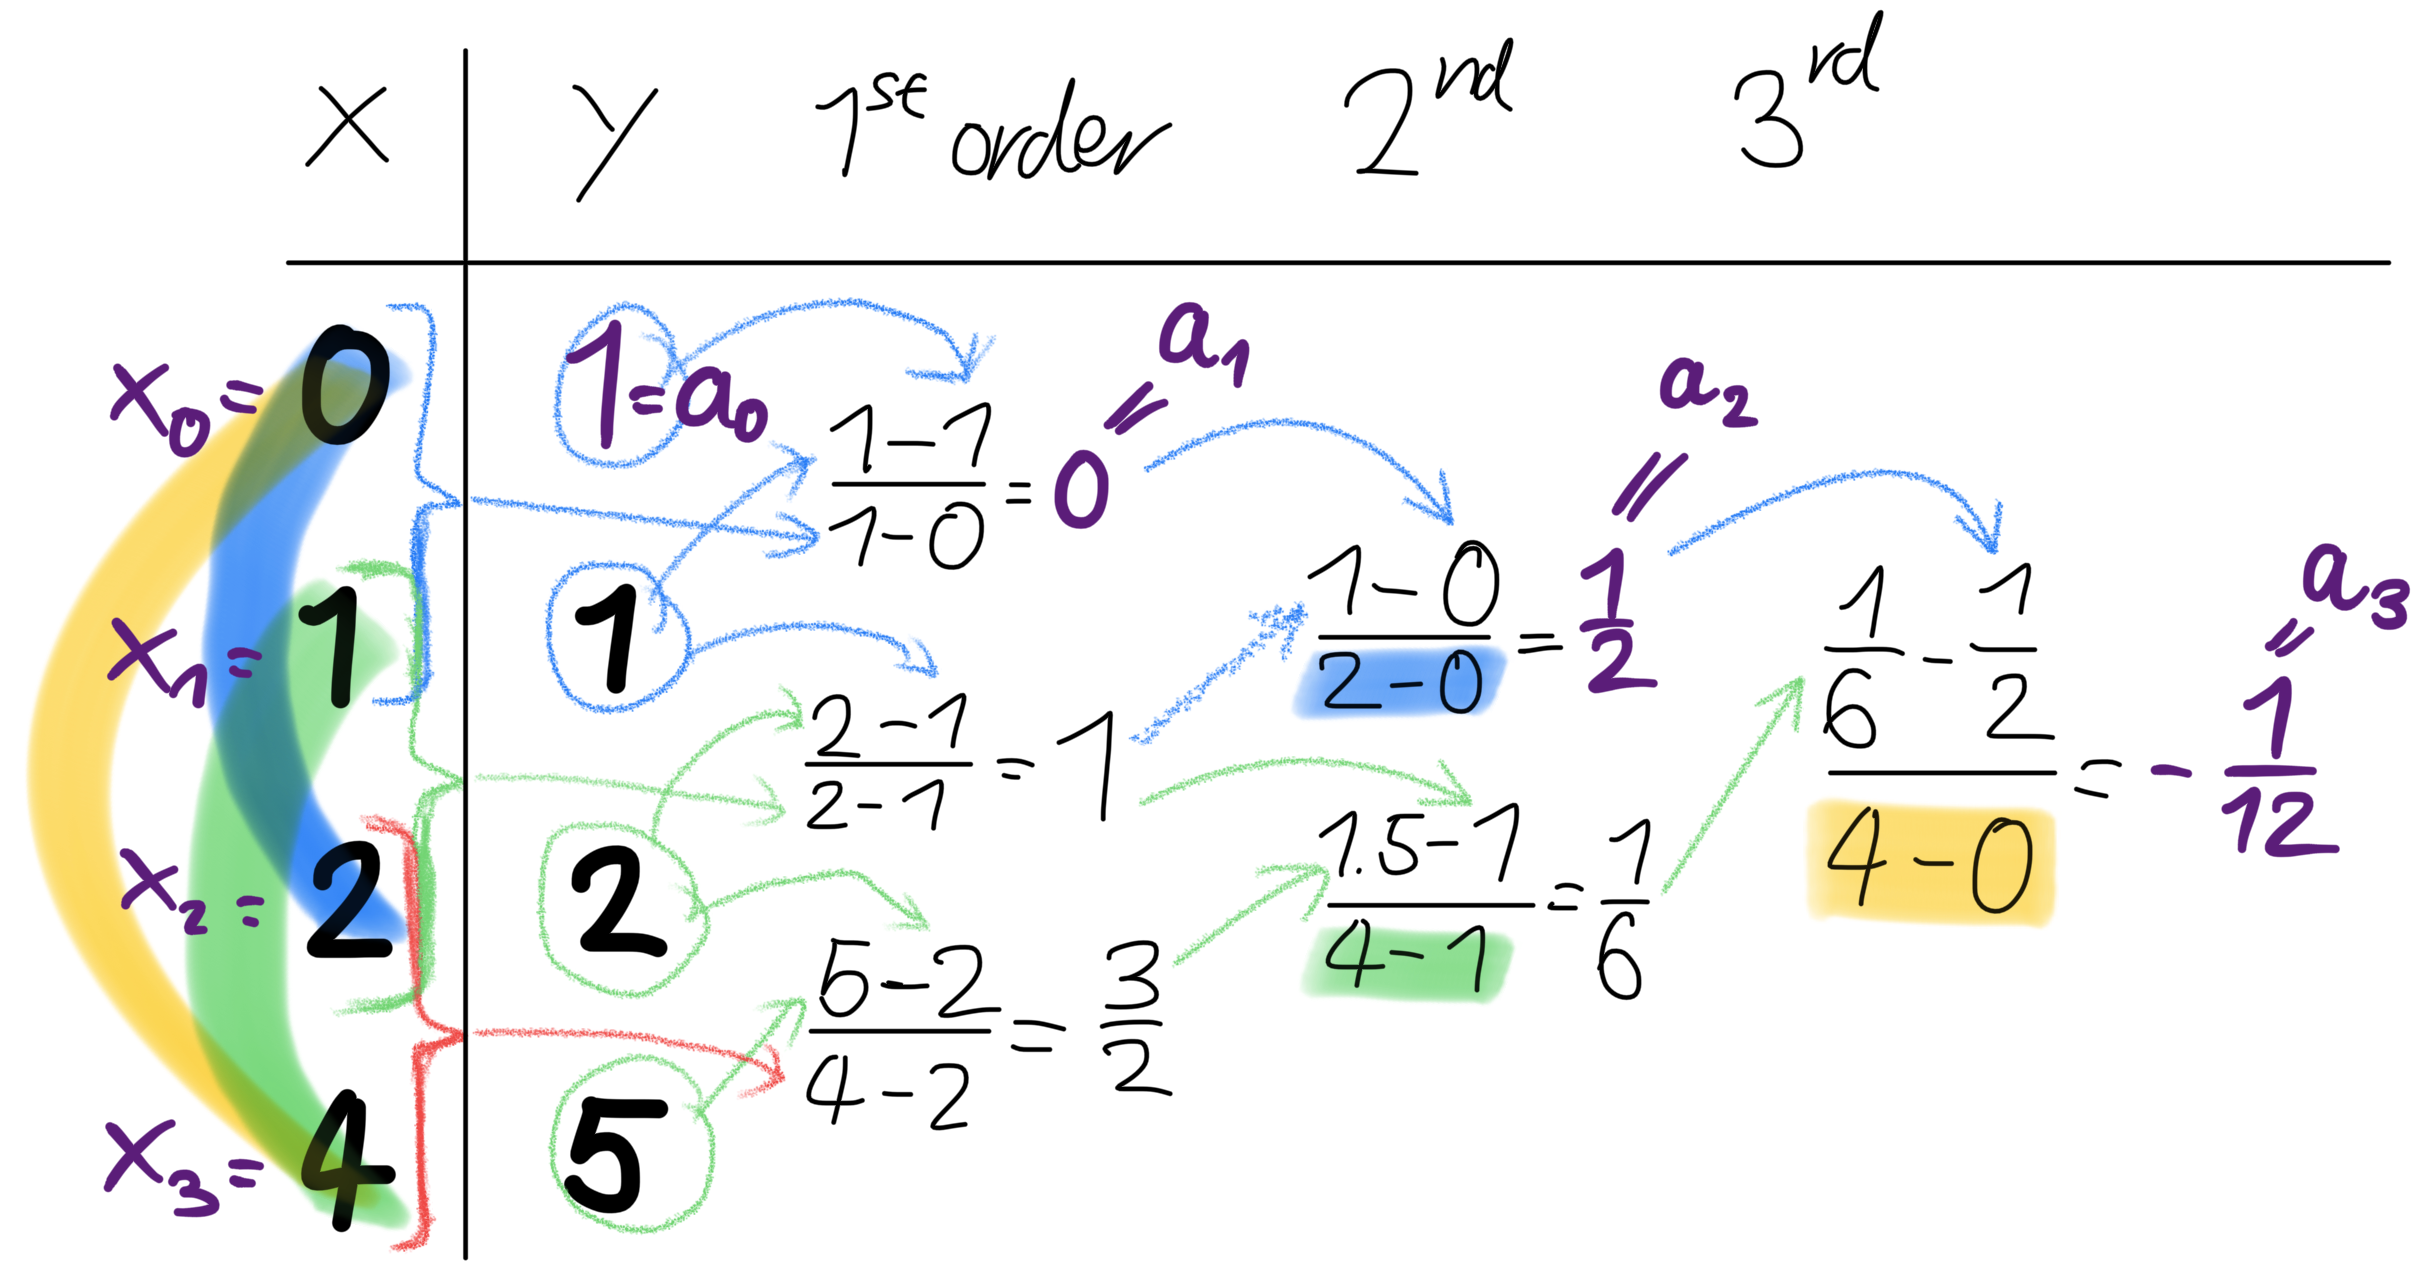
\includegraphics[width=0.6\columnwidth]{images/divided-differences}}

        \newpage
        \section{Basic Math}

\subsection{Roots}

\begin{align*}
    \sqrt[n]{a}\cdot\sqrt[n]{b} & = \sqrt[n]{a\cdot b} \\
    \frac{\sqrt[n]{a}}{\sqrt[n]{b}} & = \sqrt[n]{\frac{a}{b}} \\
    (\sqrt[n]{a})^m & = \sqrt[n]{a^m} \\
    \sqrt[m]{\sqrt[n]{a}} & = \sqrt[m\cdot n]{a}
\end{align*}

\subsection{Logarithm}

\begin{align*}
    \log_n(a\cdot b) & = \log_n(a) + \log_N(b) \\
    \log_n(a\div b) & = \log_n(a) - \log_N(b) \\
    \log_n(a^b) & = b \cdot \log_n(a)
\end{align*}

\subsection{Trigonometry}

\begin{align*}
    \tan\theta & = \frac{\sin\theta}{\cos\theta} \\
    \sin -\theta & = -\sin\theta\text{ (cos same)} \\
    \sin 2\theta & = 2\sin\theta\cos\theta \\
    \cos 2\theta & = 2\cos^2\theta - \sin^2\theta = 2\cos^2\theta - 1 = 1 - 2\sin^2\theta \\
    \sin(\alpha \pm \beta) & = \sin\alpha\cos\beta\pm\cos\alpha\sin\beta \\
    \cos(\alpha\pm\beta) & = \cos\alpha\cos\beta \mp \sin\alpha\sin\beta
\end{align*}

\subsection{Binomial Coefficient}
\begin{align*}
	\binom{n}{k} = \frac{n!}{k!(n-k)!}
\end{align*}

\subsection{Faculties}
\begin{align*}
    0! = 1, 1! = 1, 2! = 2, 3! = 6, 4! = 24, 5! = 120, 6! = 720
\end{align*}

\subsection{Determinant}
\makebox[\columnwidth]{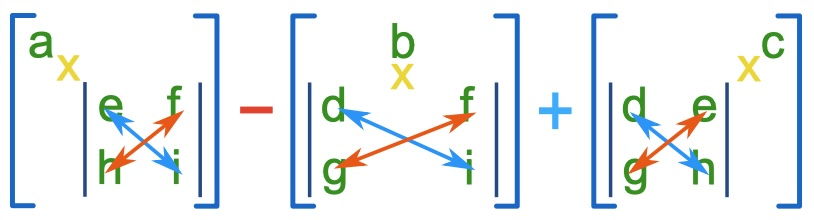
\includegraphics[width=0.5\columnwidth]{images/determinant}}

\begin{align*}
	\det
	\begin{bmatrix}
		a & b \\
		c & d
	\end{bmatrix}
	=
	ad-bc
\end{align*}
\begin{align*}
	\det
	\begin{bmatrix}
		a & b & c \\
		d & e & f \\
		g & h & i
	\end{bmatrix}
	=
	a(ei-fh)-b(di-fg)+c(dh-eg)
\end{align*}

\makebox[\columnwidth]{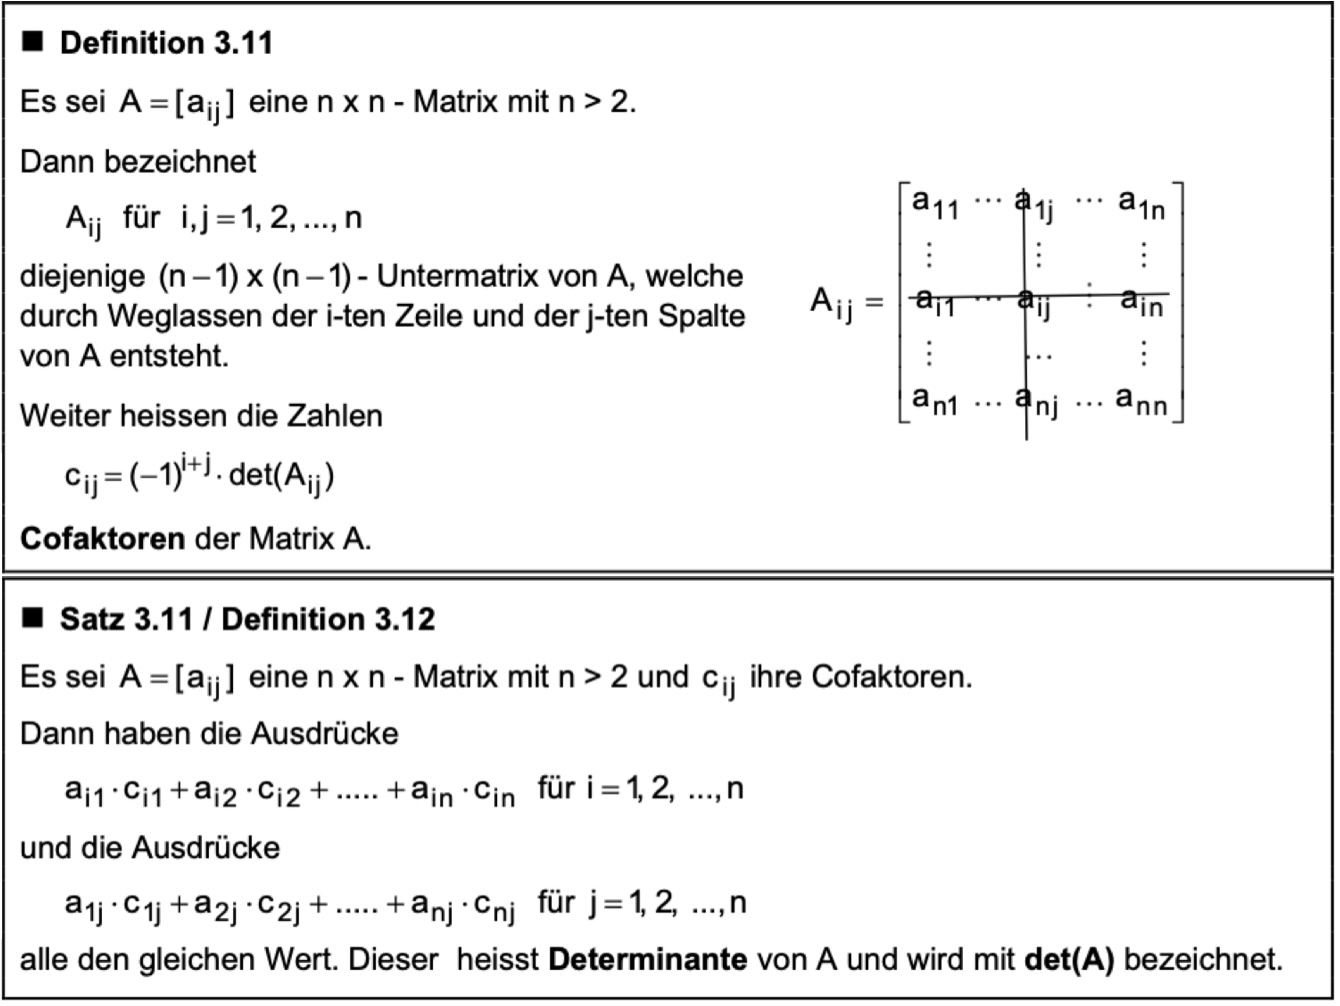
\includegraphics[width=\columnwidth]{images/determinant2}}

\subsubsection{Properties}
\begin{itemize}
	\item $\det\left(A^{-1}\right) = \frac{1}{\det(A)}$
	\item $\det(A^T) = \det(A)$
	\item $\det(I) = 1$
	\item $\det(cA) = c^n\det(A)\quad(\text{for an }n\times n\text{ matrix})$
	\item $\det(AB) = \det(A)\det(B)$
	\item $\det(A) = \prod_{i=1}^n \lambda_i$
\end{itemize}

\subsection{Derivatives}
\begin{tabular}{r|l}
    $f(x)$                & $\frac{df}{dx}$                 \\
    \hline
    $\sinh(x)$            & $\cosh(x)$                      \\
    $\cosh(x)$            & $\sinh(x)$                      \\
    $\mathrm{arcsinh}(x)$ & $1 \div \sqrt{x^2+1}$           \\
    $\mathrm{arccosh}(x)$ & $1 \div \sqrt{x^2 - 1}$ ($1<x$) \\
    $\tan(x)$             & $\cos^{-2}(x)$                  \\
    $\log(x)$             & $x^{-1}$
\end{tabular}

\subsection{Integrals}
\begin{tabular}[h]{rl}
    $\int x^n\ dx$               & $= \frac{1}{n+1}x^{n+1} + C$             \\
    $\int \frac{1}{x}\ dx$       & $= \ln |x| + C$                          \\
    $\int \frac{1}{ax + b}\ dx$  & = $\frac{1}{a} \ln |ax+b| + C$           \\
    $\int \frac{1}{(x+a)^2}\ dx$ & $= -\frac{1}{x+a} + C$                   \\
    $\int \frac{1}{1 + x^2}$     & $= \tan^{-1} x + C$                      \\
    $\int \ln ax\ dx$            & $= x\ln ax - x + C$                      \\
    $\int e^{ax}\ dx$            & $= \frac{1}{a} e^{ax} + C$               \\
    $\int \sin(ax)\ dx$          & $= -\frac{1}{a}\cos(ax) + C$             \\
    $\int \sin^2(ax)\ dx$        & $= \frac{x}{2}-\frac{\sin(2ax)}{4a} + C$ \\
    $\int x\cos x\ dx$           & $= \cos x + x\sin x + C$                 \\
    $\int \sinh(ax)\ dx$         & $= a^{-1}\cosh{ax} + C$                  \\
    $\int \cosh(ax)\ dx$         & $= a^{-1}\sinh{ax} + C$                  \\
\end{tabular}

\subsection{Integration Techniques}

\subsubsection{Integration by Parts}
\begin{equation*}
    \int_a^b u(x)v'(x)\ dx = \left[ u(x)v(x) \right]_a^b-\int_a^bu'(x)v(x)\ dx
\end{equation*}

Or, with $u=u(x)$, $du=u'(x)\ dx$, $v=v(x)$ and $dv=v'(x)\ dx$:
\begin{equation*}
    \int u\ dv=uv - \int v\ du
\end{equation*}

\subsubsection{Substitution}
\begin{equation*}
    \int_a^b f(g(x))\cdot g'(x)\ dx = \int_{g(a)}^{g(b)}f(u)\ du
\end{equation*}

\subsubsection{Leibniz Integral Rule}
\begin{multline*}
    \frac{d}{dx}\left(\int_{a(x)}^{b(x)}f(x,t)\ dt\right)
    =
    \\
    f(x,b(x))\cdot\frac{d}{dx}b(x)
    -f(x,a(x))\cdot\frac{d}{dx}a(x)
    +\int_{a(x)}^{b(x)}\frac{\partial}{\partial x}f(x,t)\ dt
\end{multline*}
Special case where $a(x)=a=\mathrm{const.}$ and $b(x)=b=\mathrm{const.}$:
\begin{equation*}
    \frac{d}{dx}\left(\int_a^b f(x,t)\ dt\right)
    =\int_a^b\frac{\partial}{\partial x}f(x,t)\ dt
\end{equation*}

\subsection{Converting second-order ODEs}

For a second-order equation $y''=f(x,y,y')$, we can introduce $p=y'$, transforming the equation
to $p'=f(x,y,p)$ and thus receiving a system of ODEs with initial conditions
$p(x_0)=y_1, y(x_0) = y_0$.

    \end{multicols}
\end{document}
